For both sampling methods, we use a helper function to compute the
radical inverse and a precomputed list of the first 12 prime numbers,
one for each sampling dimension
(\emph{Monte Carlo II}, slides~19--20).

\lstinputlisting[
    language=C++,
    firstline=13,
    lastline=27,
    firstnumber=13
]{../../assignments/sampler/halton.cpp}

\textbf{Halton.}

We track the number of calls to \texttt{next2D()} and
\texttt{next1D()} separately for each path. Successive calls use
different Halton dimensions: \texttt{next2D()} uses dimension pairs
$(1,2)$, $(3,4)$, $(5,6)$, and $(7,8)$, while \texttt{next1D()}
uses dimensions $9$, $10$, $11$, and $12$. After the fourth call
to either method, that method switches to independent sampling
for the remainder of the path.

Between paths, we reset both call counters and increment the
Halton sample index. When rendering a new pixel, we reset the
sample index to zero.

\lstinputlisting[
    language=C++,
    firstline=31,
    lastline=94,
    firstnumber=31
]{../../assignments/sampler/halton.cpp}

\textbf{Halton with Cranley--Patterson rotation.}

Unlike the vanilla Halton implementation, we generate a random
vector $\mathbf{V}\in[0,1)^{12}$ at each call to \texttt{generate()},
with one independently sampled value per dimension. This gives
each pixel a different rotation vector, which remains fixed
for all paths within that pixel.

For dimension $d$, we add the corresponding component $V_d$
to the Halton value and take the result modulo one:
\[
\widetilde{x}_{i,d}
= \bigl(\phi_{b_d}(i) + V_d\bigr) \bmod 1,
\]
where $b_d$ is the prime base associated with dimension $d$ and
$i$ is the path index within the pixel.

\lstinputlisting[
    language=C++,
    firstline=31,
    lastline=104,
    firstnumber=31
]{../../assignments/sampler/halton_decorr.cpp}

\begin{figure}[htbp]
    \centering
    \begin{minipage}[t]{0.32\textwidth}
        \centering
        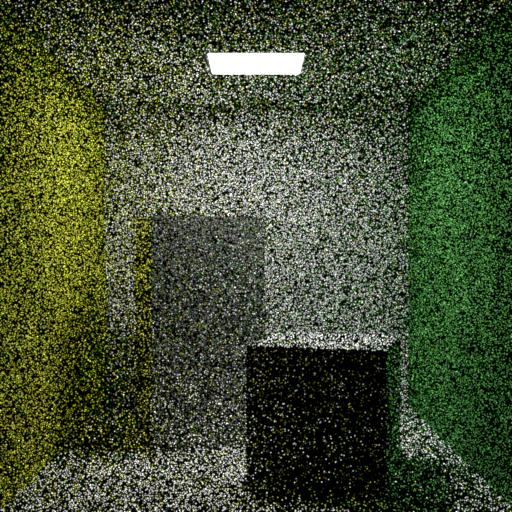
\includegraphics[width=\linewidth]{pictures/cbox-path.png}
        \par\small Independent sampling
    \end{minipage}
    \hfill
    \begin{minipage}[t]{0.32\textwidth}
        \centering
        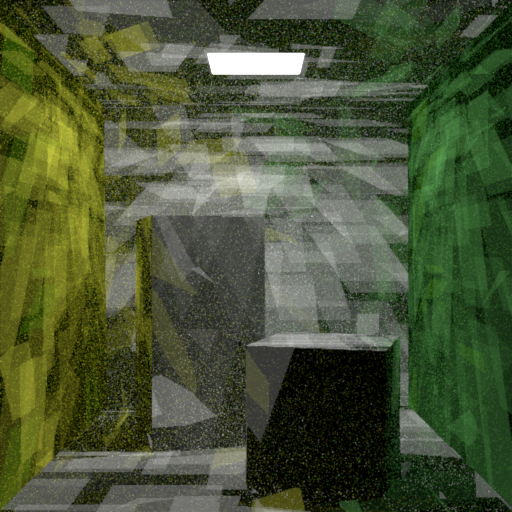
\includegraphics[width=\linewidth]{pictures/cbox-path-halton.png}
        \par\small Vanilla Halton sampling
    \end{minipage}
    \hfill
    \begin{minipage}[t]{0.32\textwidth}
        \centering
        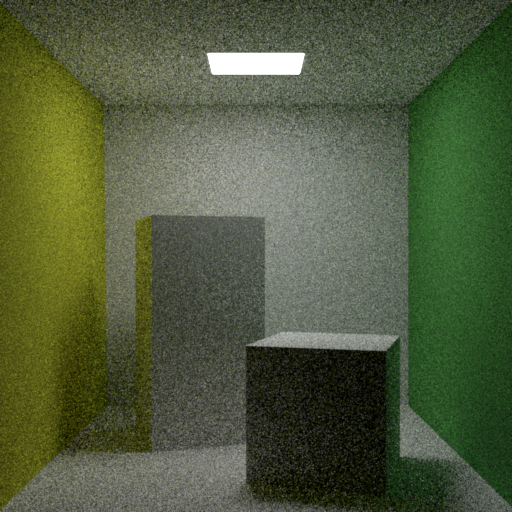
\includegraphics[width=\linewidth]{pictures/cbox-path-halton-decorr.png}
        \par\small Decorrelated Halton sampling
    \end{minipage}
    \caption{Comparison of independent, vanilla Halton, and decorrelated
    Halton sampling. Vanilla Halton sampling produces large, structured
    artifacts due to correlations between pixels. With Cranley--Patterson
    rotation, these artifacts are no longer apparent, and the image
    appears slightly less noisy than the independently sampled render.}
    \label{fig:halton-rendering}
\end{figure}